\section{Einführung}

\begin{frame}{Unser Kurs}
  \begin{itemize}
    \item In \LaTeX\ gibt es immer viele Möglichkeiten, ein Ziel zu erreichen
    \item Wir zeigen einen modernen Ansatz
    \item Wir erklären, warum wir diesen Ansatz gewählt haben
    \item Weitere Ansätze werden an manchen Stellen kurz erwähnt
  \end{itemize}
\end{frame}

\begin{frame}{Was ist \LaTeX?}
  \begin{itemize}
    \item \emph{Programmiersprache} zum Setzen von Text
    \item Kein WYSIWYG, es werden Befehle und Inhalt in normale Text-Dateien geschrieben.
    \item Kompiler überträgt \LaTeX-Code in ein Ausgabedokument (meist PDF)
    \item Open-source mit zahlreichen Erweiterungsmöglichkeit (Pakete)
  \end{itemize}
\end{frame}

\begin{frame}{Warum \LaTeX?}
  \begin{itemize}
    \item Hervorragender Text- und Formelsatz
    \item Automatisierte Erstellung von Inhalts- und Literaturverzeichnis
      \begin{itemize}
        \item Oder auch: Tabellenverzeichnis, Abbildungsverzeichnis, Index, Glossar, Abkürzungen, Definitionen, …
      \end{itemize}
    \item \TeX-Dateien sind reine Text-Dateien
      \begin{itemize}
        \item[$\Rightarrow$] Gut für Versionskontrolle geeignet
      \end{itemize}
    \item Sehr gute Vorlagen für wissenschaftliches Arbeiten
      \begin{itemize}
      \item Aber auch: Briefe, Notensatz, Präsentationen (auch diese)
      \end{itemize}
    \item Ausgezeichnete Dokumentation
    \item Erweiterbar durch zahlreiche und mächtige Pakete
    \item Auf allen geläufigen Betriebssystemen verfügbar
    \item Ausgabe direkt als PDF mit Hyperlinks
  \end{itemize}
\end{frame}

\begin{frame}{Geschichte}
  \begin{columns}
    \begin{column}{0.73\textwidth}
      \TeX:
      \begin{itemize}
        \item Geschrieben von Donald E. Knuth 1978, um sein Buch \enquote{The Art of Computer Programming} zu setzen
        \item Auf Aussprache achten!
        \item Version (2014): $3.14159265 → \mathup{π}$
        \item Viele Erweiterungen: \eTeX, pdf\TeX, \XeTeX, \LuaTeX
      \end{itemize}

      \vspace{10pt}
      \LaTeX:
      \begin{itemize}
        \item Geschrieben von Leslie Lamport 1984
        \item Version (1994): \LaTeXe
        \item \LaTeX3 seit Anfang der Neunziger in Arbeit…
      \end{itemize}
    \end{column}
    \begin{column}{0.23\textwidth}
      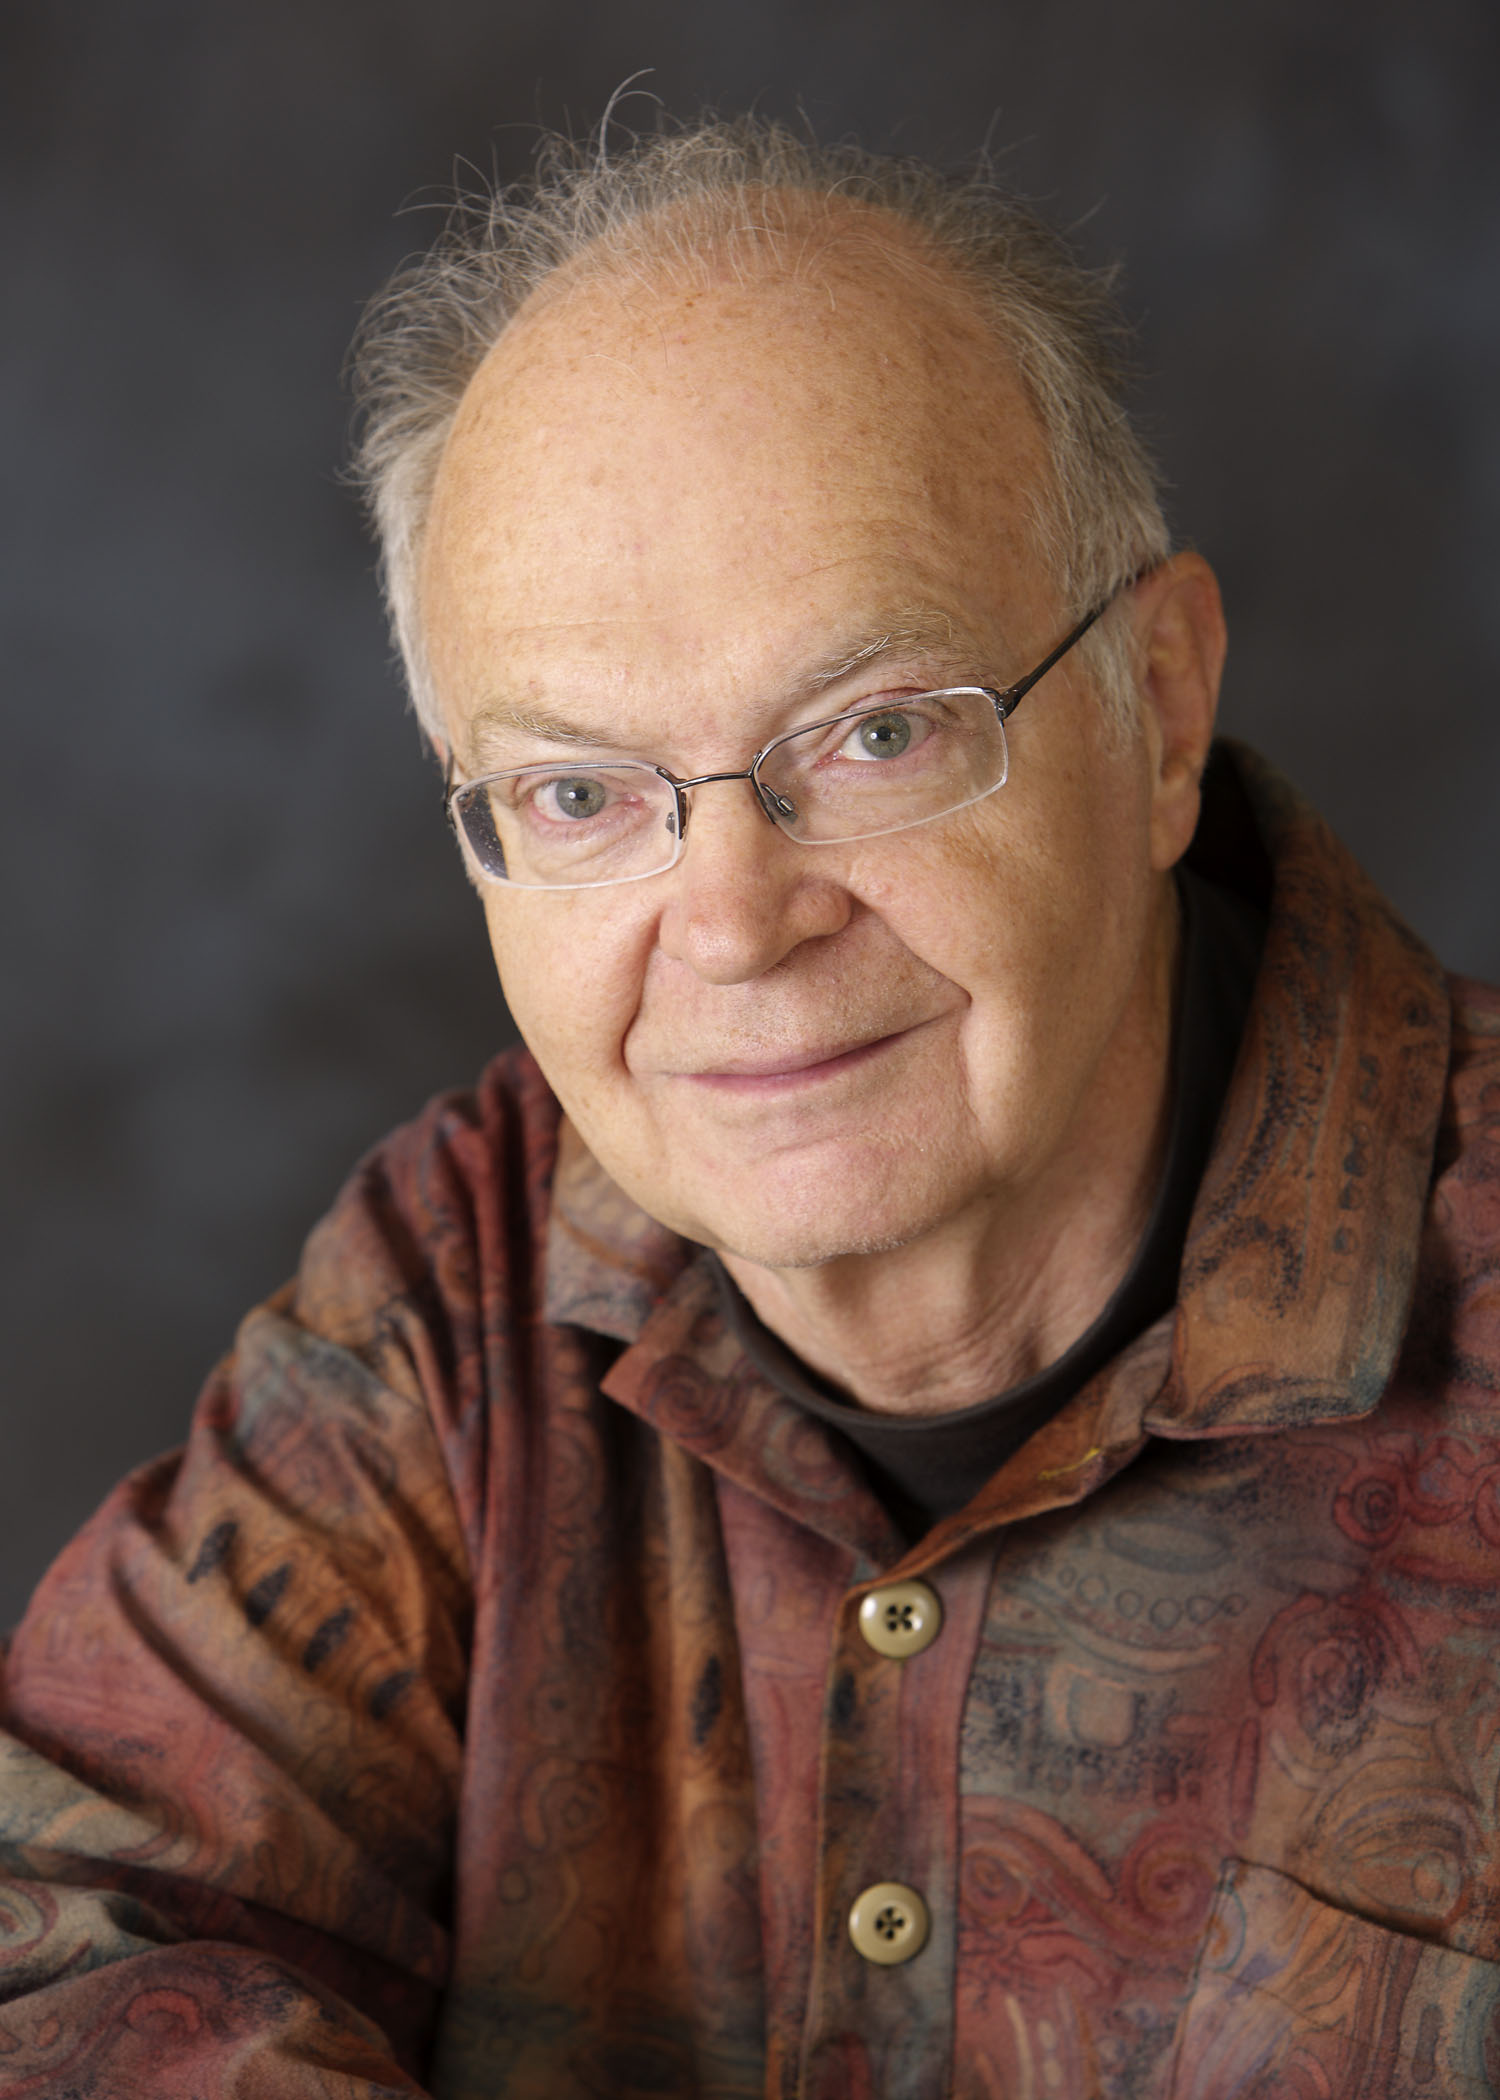
\includegraphics[height=0.45\textheight]{figures/knuth.jpg}\\
      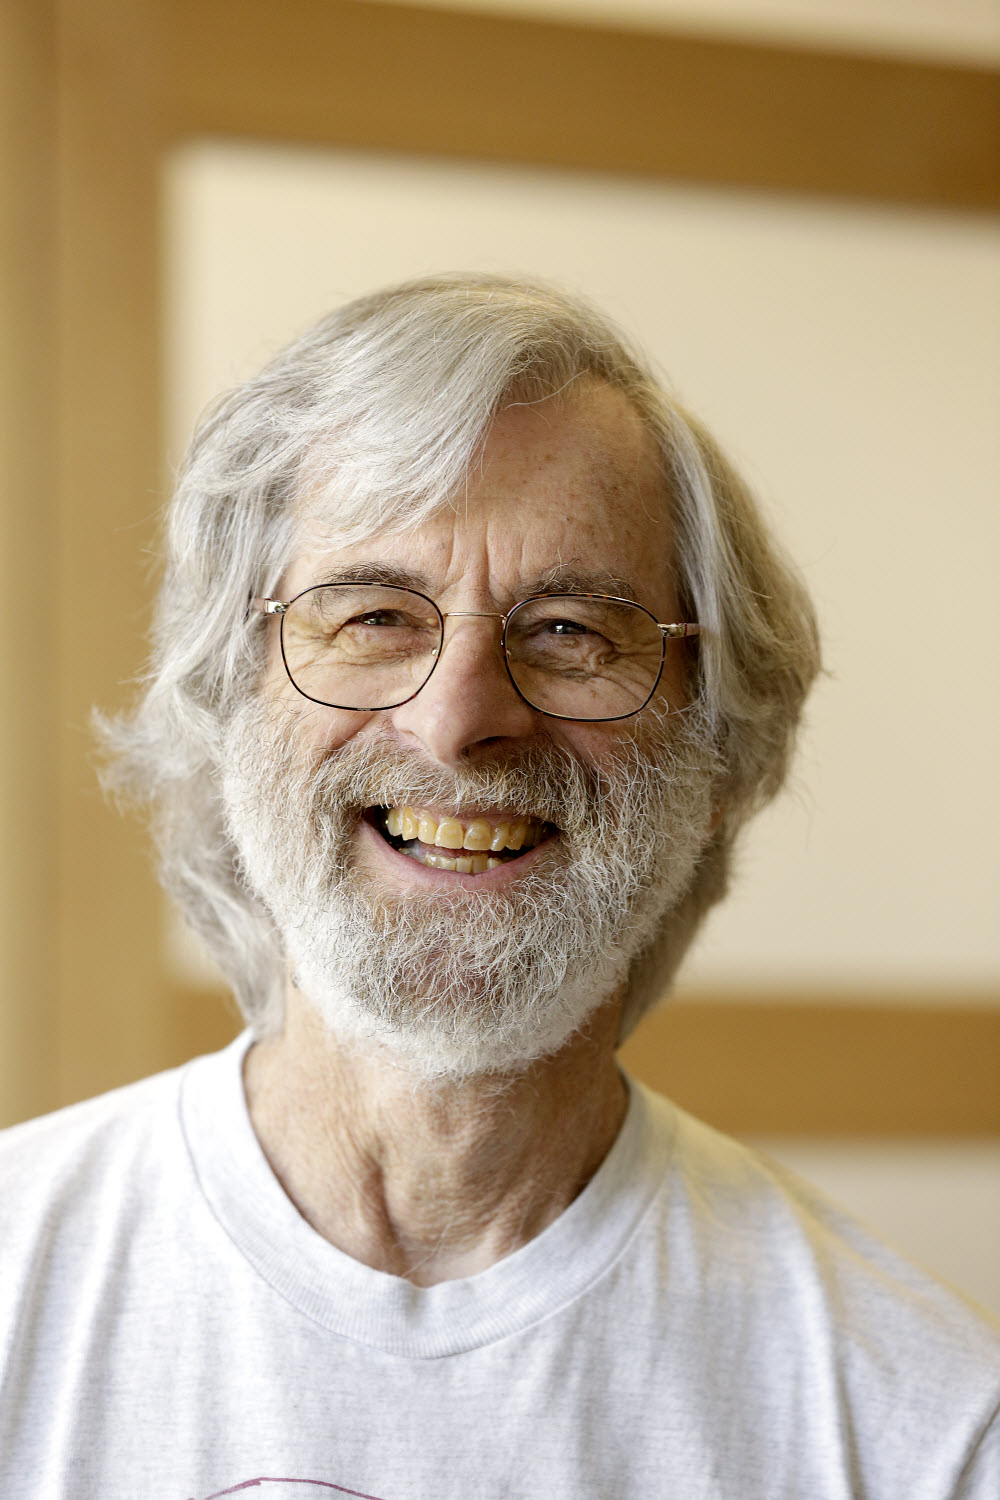
\includegraphics[height=0.45\textheight]{figures/lamport.jpg}
    \end{column}
  \end{columns}
\end{frame}

\begin{frame}{Begriffe}
  \begin{description}
    \item[\TeX-Engine] Implementierung von \TeX, wird als Programm ausgeführt
    \item[\TeX-Format] Paket, welches standardmäßig geladen wird, z.B. \LaTeX
  \end{description}

  \vspace{10pt}
  Eine Kombination davon ist oft ein neues Programm.\\[10pt]
  Beispiel: \texttt{dvilualatex} = \LuaTeX\ + \LaTeX\ + DVI-Output (statt PDF)
\end{frame}
